\subsection{Choice of equalization techniques and resolution} 
\label{ch:equalization_choice}

To evaluate the required equalization for the data link with the given channel, different options were simulated and the resulting eye-diagrams were created. \\
Figure \ref{fig:eyes_10gbs} shows the eye diagram at the RX input for different equalization configurations with the link running at \unit[10]{Gb/s} and \unit[$\pm$1]{V} TX signal swing. For \unit[2]{Gb/s} the resulting eye diagrams are presented in figure \ref{fig:eyes_2gbs}. All eyes are for a sequence of 1000 pseudo-random bits generated by a 7-bit PRBS generator.\\
Without any equalization the eye is closed for the fast case. By adding a single post cursor (2-tap TXPE) the eye gets much more relaxed. The vertical eye opening is approximately \unit[360]{mV} and the horizontal eye opening \unit[68]{ps}. Comparing this with already implemented links, e.g. the PCIe specification which allows a minimum width of \unit[0.4]{UI} and height of \unit[120]{mV} at the reciever \cite{pcie_spec} for the same BER as in this project (10$^{-12}$), it should be feasible to meet the requirements with only this equalization. As the amount of deterministic jitter for the channel is already included in the simulation, a remaining total jitter of \unit[68]{ps} can be introduced by the transmitter and receiver circuits. The required BER results in a Q of 7 and therefore maximal deterministic jitter in Rx and Tx can be approximated as $DJ\leq\unit[68]{ps}-14*RJ$. So for example we could deal with up to \unit[26]{ps} additional DJ for \unit[3]{ps} of random jitter introduced by the circuits.\\
Adding a second post cursor increases the eye opening in both directions a bit. However, this increase is relatively small for the effort required. As we want to implement a low-power link, the additional amount of power consumption required does not justify adding another tap. Using a pre instead of a post cursor leads to worse performance and is therfore not considered any further. For \unit[2]{Gb/s} with reduced signal swing the received eye is already very good even without any equalization, adding one post cursor reduces the ISI even further.\\
Adding other equalization techniques at the receiver could improve the eye opening and therefore the BER further but would also require more power, especially for DFE. As the received signal seems to be good enough with only equalization at the transmitter, we decided to use only TXPE with 2-taps (cursor and one post cursor) as equalization in the system.


%TODO other equalization techniques
%TODO other references?

\begin{figure}[H]
  \centering
  \subfigure[no equalization]
  {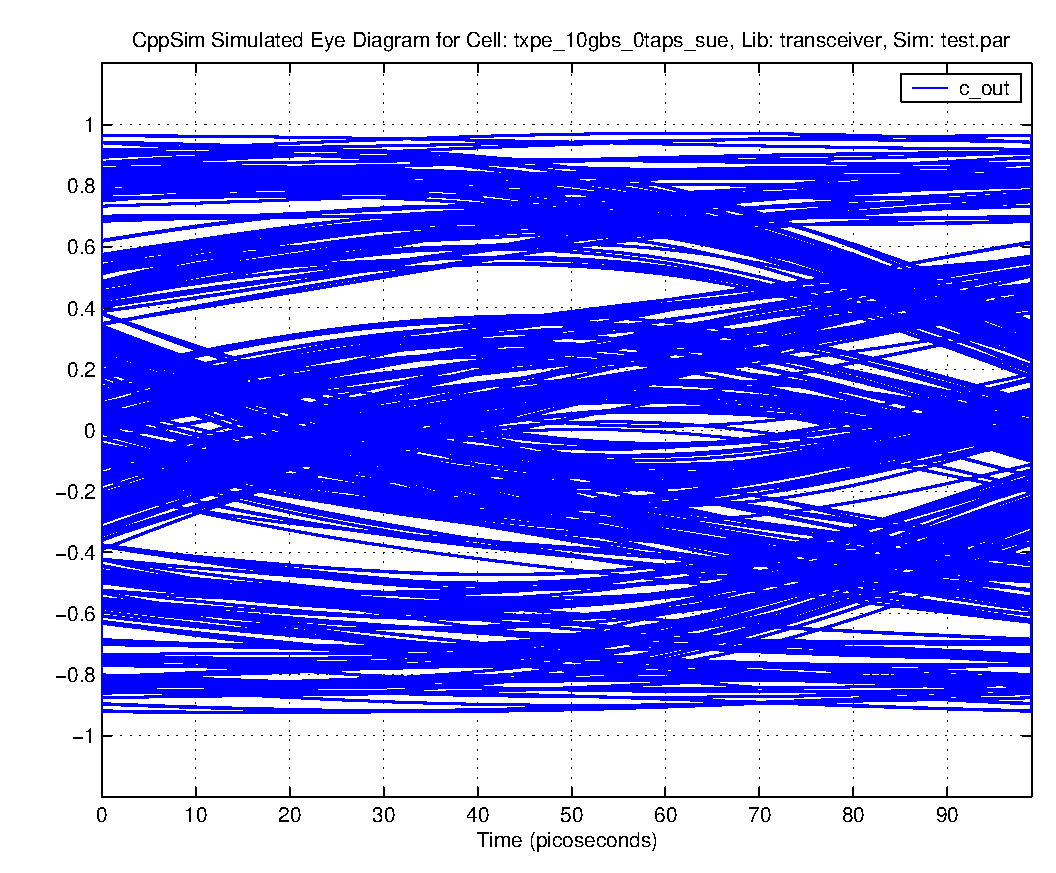
\includegraphics[scale=0.5]{eyes/eye_10gbs_0taps.eps}}
  \subfigure[TXPE, one post cursor]
  {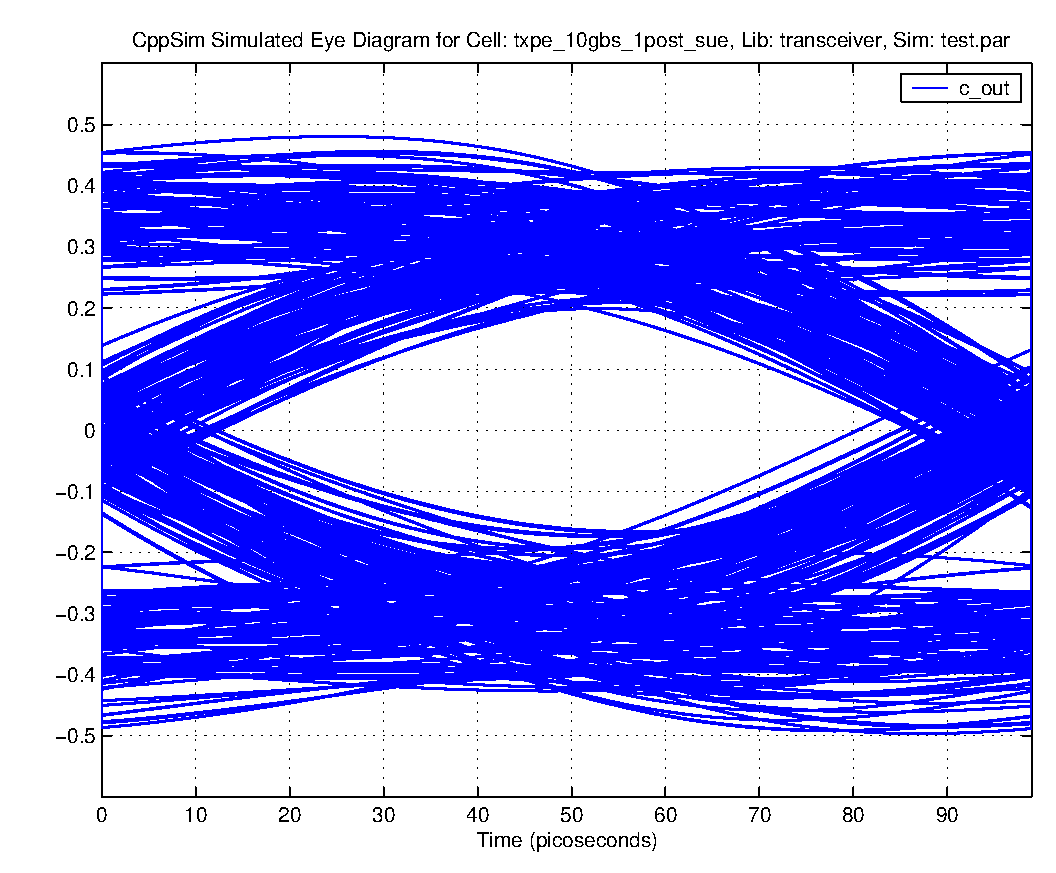
\includegraphics[scale=0.5]{eyes/eye_10gbs_1post.eps}}
  \subfigure[TXPE, two post cursors]
  {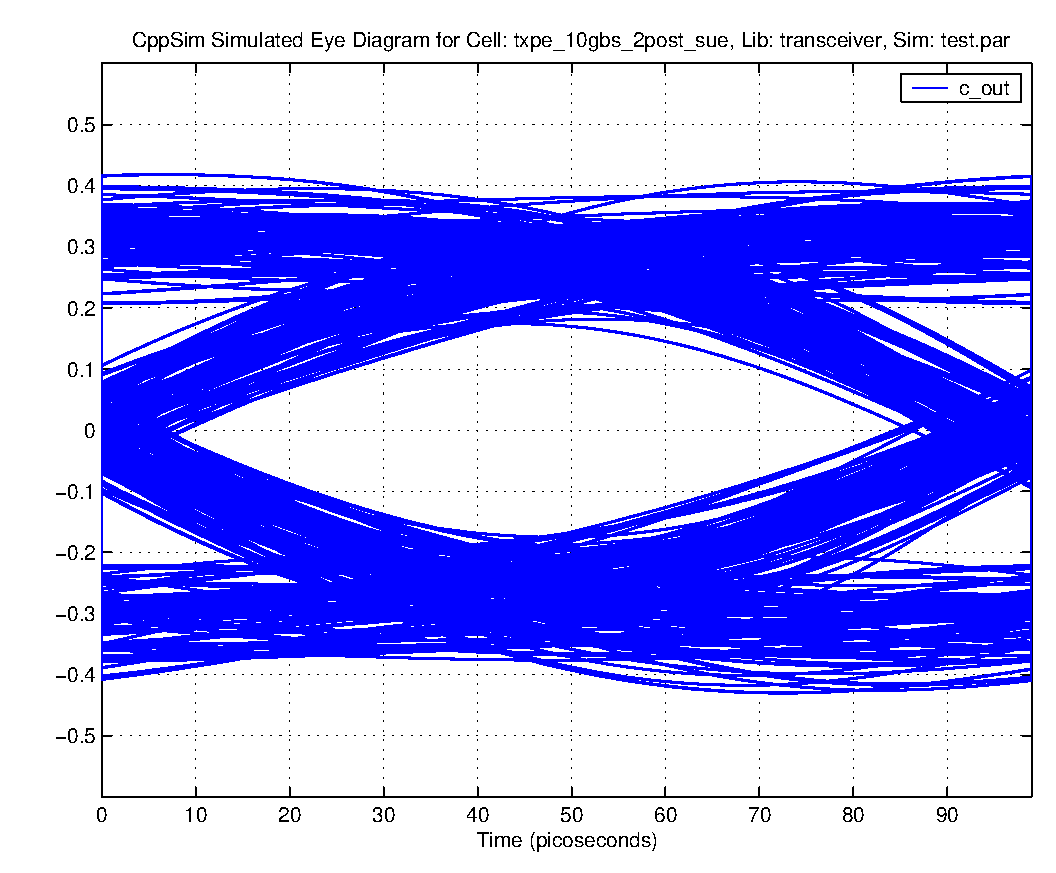
\includegraphics[scale=0.5]{eyes/eye_10gbs_2post.eps}}
  \subfigure[TXPE, one post and one pre cursor]
  {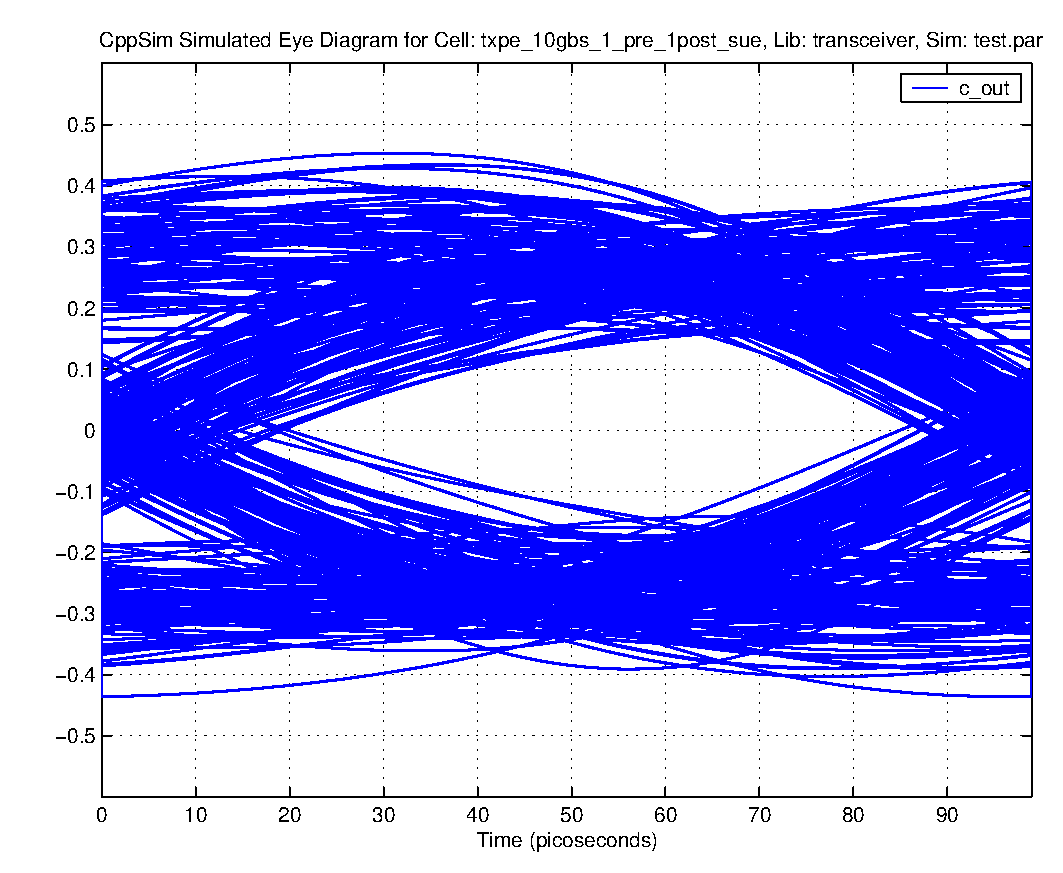
\includegraphics[scale=0.5]{eyes/eye_10gbs_1pre_1post.eps}}
  \caption{Eye diagrams for \unit[10]{Gb/s} and \unit[$\pm$1]{V} TX signal swing}
  \label{fig:eyes_10gbs}
\end{figure}

\begin{figure}[H]
  \centering
  \subfigure[no equalization]
  {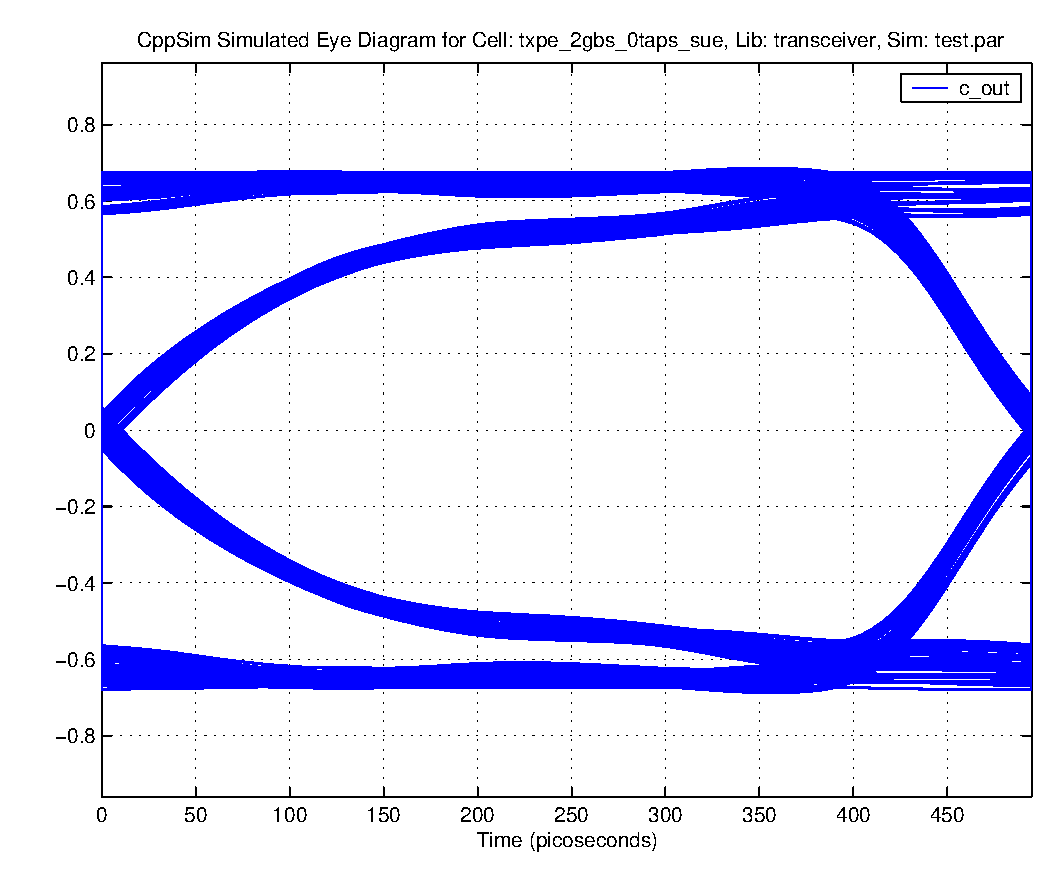
\includegraphics[scale=0.5]{eyes/eye_2gbs_0taps.eps}}
  \subfigure[TXPE, one post cursor]
  {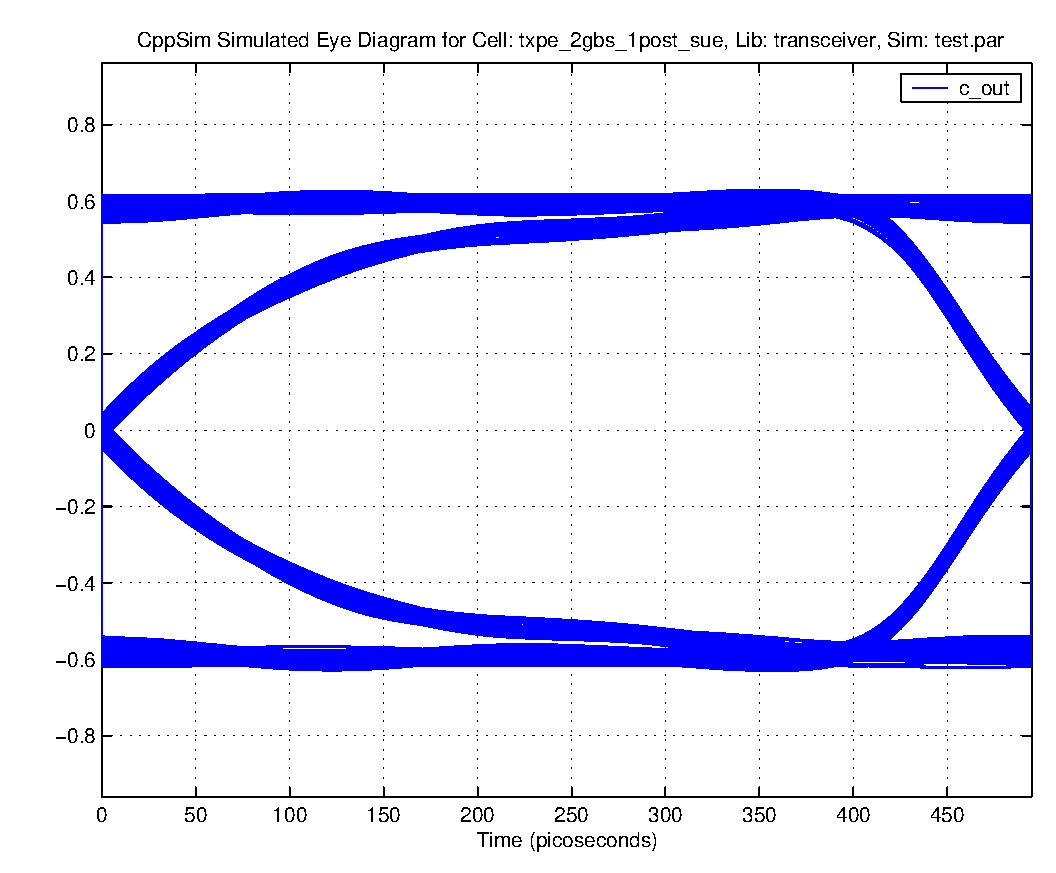
\includegraphics[scale=0.5]{eyes/eye_2gbs_1post.eps}}
  \subfigure[TXPE, two post cursors]
  {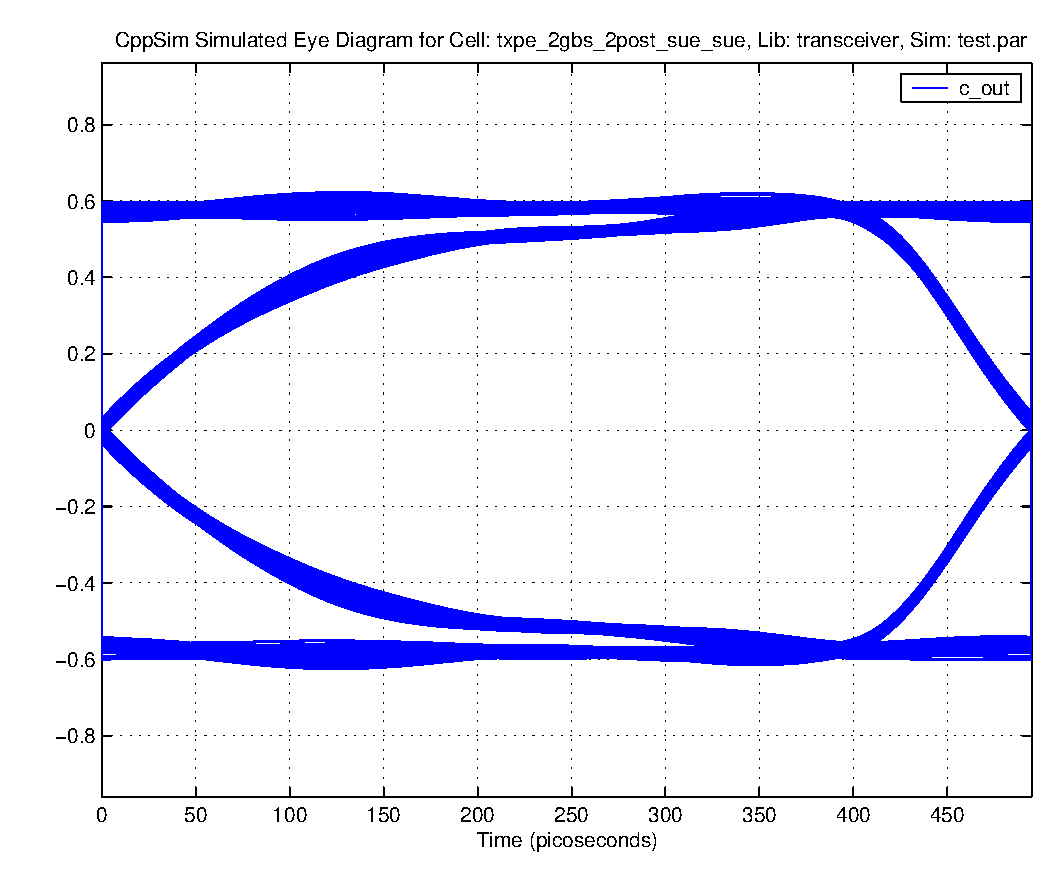
\includegraphics[scale=0.5]{eyes/eye_2gbs_2post.eps}}
  \caption{Eye diagrams for \unit[2]{Gb/s} and \unit[$\pm$0.7]{V} TX signal swing}
  \label{fig:eyes_2gbs}
\end{figure}